\documentclass[../main/main.tex]{subfiles}

\newdate{date}{20}{03}{2020}

\begin{document}

\marginpar{ \textbf{Lecture 4.} \\  \displaydate{date}. \\ Compiled:  \today.}

Let us consider the more common case of metals. A metal is constituted by free atoms merged into a solid. In particular, our system is constituted by nuclei, core electrons and ions (nuclei+core electrons) with mass \( M \) and charge  \( +Ze \). In a metal, while the core electrons remain rather closer to their nuclei, the so called "valence electrons" become very free and they are spread over all the system. Each valence electron has mass \( m \) and charge \( -e \).



In a real metal the electron lattice potential is as in Fig. \ref{fig:4_1}. We have a characteristic behaviour due to the fact that electrons must move subject to the periodic potential made by positive ions. Now, in the Jellium model we make the drastic approximation to replace the periodic potential with a uniform positive background and so also the potential becomes smeared out. Hence, while in a real metal the positive charge is localized (for instance in the ionic coarse and crystal lattice), in the Jellium model the charge is uniform.  \marginpar{
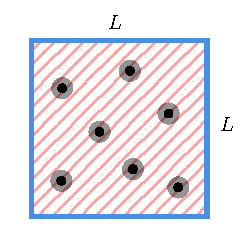
\includegraphics[width=\marginparwidth]{../lessons/4_image/1.pdf}
\captionof{figure}{\label{fig:} Cubic metal of volume \( L \): nuclei are represented in black, core lectrons in grey and valence electron with the red pattern. }
}


\begin{figure}[h!]
\begin{minipage}[c]{0.5\linewidth}
\subfloat[][Real (metal) lattice periodic potential.]{ 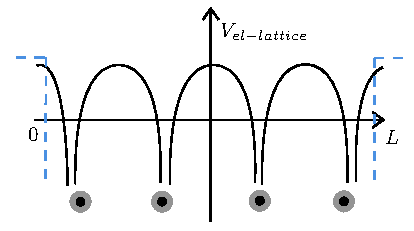
\includegraphics[width=0.85\textwidth]{../lessons/4_image/2.pdf}  \label{fig:4_1} }
\end{minipage}
\begin{minipage}[]{0.5\linewidth}
\centering
\subfloat[][Jellium model potential.]{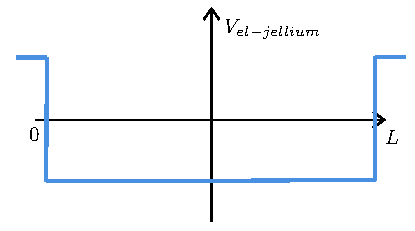
\includegraphics[width=0.85\textwidth]{../lessons/4_image/3.pdf}  \label{fig:4_2} }
\end{minipage}
\caption{\label{fig:} }
\end{figure}

Moreover, we know that if the temperature is finite, also the ions vibrate and even at zero temperature there is the zero point energy.
However, we completely neglect the ionic dinamical motion so this means that for instance we have no phonons and no lattice vibrations because only the electrons are the real dynamical variables.
We also assume that we are in the thermodynamic limit, so the number of particle of electrons is very large and also the volume of the system (a cubic box) is very large, in such a way that the particle density is constant and finite.

Let us resume the drastic approximations involved in this model: \marginpar{Drastical assumptions}
\begin{itemize}
\item in real metals (or in a plasma) the positive charge is not uniform, but localized in the ionic cores ("crystal lattice"). In Jellium, the positive charge is uniform distributed. The assumption of a uniform background is drastic and for this reason the present model can provide only a qualitative account of real metals.
\item No dynamical motion of the positive charges (no phonons, namely lattice vibrations...), indeed the positive ions are much heavier than the electrons and it is permissible to neglect the ionic motion entirely. The dynamic motion is only the one of electrons.
\item We assume thermodynamic limit: \( N \rightarrow \infty  \), namely \( V = L^3 \rightarrow \infty  \) (cubic box of side \( L \)) and with the particle density \( n=N/V \) constant.
\end{itemize}

Let us write formally the total Hamiltonian of this system:
\begin{equation}
  \hat{H} = \hat{H}_b + \hat{H}_{el-b} + \hat{H}_{el}
\end{equation}
where \( H_b \) describes the positive background energy, the \( \hat{H}_{el-b} \) the interaction between the electrons and positive background and the term relative to electrons \( \hat{H}_{el} = \hat{T} + \hat{V}  \) which has a kinetic term and a potential term which describes the electrons-electrons interaction.  The last one is the most
diffigult part of our \( N\)-body problem.

For simplicity since we are working with the coulomb interaction, we assume the GS unit system, namely:
\begin{equation*}
  \frac{1}{4 \pi \varepsilon _0} \rightarrow 1
\end{equation*}
and we define also the \textbf{charge density} \( \rho (\va{x}) \) as a function of the \textbf{number density} \( n(\va{x}) \):  \marginpar{Charge density}
\begin{equation}
  \rho (\va{x}) = e n (\va{x})
\end{equation}
Now, let us find the explicit expression for all the terms of the Hamiltonian in second quantization formalism.

\subsubsection{Positive background Hamiltonian: \( \mathbf{\hat{H}_b } \) }
Let us start in trying to find the explicit expression for the positive background hamiltonian. It is easy to see that in principle \( \hat{H}_b \) should be an operator, but actually is a purely \( c \)-number since the only dynamical variables are the electrons. Indeed, the interaction energy due to the positive background is just given by the usual electrostatic formula, where we have considered the Coulomb interaction:
\begin{equation*}
  \hat{H}_b = H_b = \frac{1}{2} \int_{V}^{} \int_{V}^{} \dd[3]{x}  \dd[3]{x'} \frac{\rho _b (\va{x}) \rho _b (\va{x}')}{\abs{\va{x}-\va{x}'} }
\end{equation*}
Hence, by using the definition of \( \rho  \):
\begin{equation*}
\begin{split}
  H_b &= \frac{e^2}{2} \int_{V}^{} \int_{V}^{} \dd[3]{x}  \dd[3]{x'}
  \frac{n_b (\va{x}) n_b (\va{x}')}{\abs{\va{x}-\va{x}'} } \\
  & \underset{\substack{n_b (\va{x}) = n = \frac{N}{V} \\ \va{y} \equiv \va{x}-\va{x}' } }{=}  \frac{e^2 n^2}{2}  \int_{V}^{} \dd[3]{x}  \int_{V}^{}  \dd[3]{y}  \frac{1}{y}
  =4 \pi V \frac{e^2 n^2}{2} \int_{0}^{\infty } \dd[]{y} y \rightarrow \infty
\end{split}
\end{equation*}
where in the second step we have changed the variable in \( \va{y} \) (since is an infinite system is not a problem).
We can immediately see that the integral diverge. It is a mathematical divergence, which reflects the fact that the Coulomb interaction is a long range interaction: it means that in our system every portion of the positive uniform background interact with every other portion of the same background and if we take into account all these contribution we get a divergence.
Remind that, for the moment, we are just taking into account the first contribution of the Hamiltonian: the idea is that since the whole system is neutral, divergencies should disappear if we consider all the components.

In order to make the expression mathematically well defined at every step of the derivation we adopt a trick, we introduce an \textbf{artificial exponential convergence factor}: \marginpar{Exponential convergence factor}
\begin{equation*}
  \frac{e^2}{x} \rightarrow \frac{e^2}{x} e^{- \mu x}
\end{equation*}
where the constant \( \mu > 0 \). The idea is that at the end of the derivation since we want to recover the real Coulomb interaction, we have to take this term \( \mu \rightarrow 0 \) in such a way \( e^{- \mu x} \rightarrow 1 \). However, before to take the limit we should take the thermodynamic limit. The order of these steps is important:
\begin{enumerate}
\item Take the thermodynamic limit \( L \rightarrow \infty, V \rightarrow \infty   \).
\item Take the limit \( \mu \rightarrow  0\).
\end{enumerate}
It means that at every step we assume the effective range of the modified Coulomb interaction (the inverse of \( mu \) is a length!) is lower than the total size of the system:
\begin{equation*}
  \frac{1}{\mu }\ll L
\end{equation*}
Namely, it is no longer true that every positive portion interact with all the other positive portions. We can shift the origin of the integration freely, apart from surface corrections which are neglected, because we are interested in only bulk properties.
Hence:
\begin{equation}
\begin{split}
H_b  &= 4 \pi V \frac{e^2 n^2}{2} \int_{0}^{\infty} \dd[]{y} y e^{- \mu y}    =  4 \pi V \frac{e^2 n^2}{2} \qty[- \eval{ \cancel{\frac{y e^{- \mu y} }{\mu }} }_0^\infty   + \frac{1}{\mu } \int_{0}^{\infty} \dd[]{y} e^{- \mu y} ]   \\
&= 4 \pi V \frac{e^2 n^2}{2} \qty[- \frac{1}{\mu ^2} e^{- \mu y} ]_0^\infty  =  4 \pi V \frac{e^2 n^2}{2} \frac{1}{\mu ^2}
\underset{n=\frac{N}{V}}{=}  \frac{1}{2} e^2 \frac{N^2}{V} \frac{4 \pi }{\mu ^2} > 0
\end{split}
\end{equation}
the integral is easily evaluated solved by parts. The final result is positive and consistent with what we expected: it should describe the repulsion between positive charges and in the limit \( \mu  \rightarrow 0 \) we recover the divergence found before (every element of charge interacts with every other one).

\subsubsection{Interaction term between electrons and background: \( \mathbf{\hat{H}_{el-b} } \) }
Let us analyze the interaction term between the particles and the background. Clearly, also in this case, we should have in principle a \( 1 \)-body operator   (electrons interact with an external field), but as we will see also we get a c-number. First, we write the electrostatic interaction between the electronic charge distribution and uniform positive one. Then, we introduce the exponential factor, we use the definition of electron density \( n_{el} \):
\begin{equation}
  n_{el}(\va{x}') = \sum_{i=1}^{N} \delta (\va{x}'-\va{r}_i)
\end{equation}
and we remember that he positive charge distribution is a constant \( n_b (\va{x})= n = N/V \). Making these substitution we obtain:
\begin{equation*}
\begin{split}
  \hat{H}_{el-b} &= H_{el-b} = - e^2 \int_{V}^{} \int_{V}^{} \dd[3]{x} \dd[3]{x'} \frac{n_{el} (\va{x}') n_b (\va{x}) }{\abs{\va{x}-\va{x}'}  } e^{-\mu \abs{\va{x}-\va{x}'} } \\
  &= - e^2 \sum_{i=1}^{N} \frac{N}{V} \int_{V}^{} \dd[3]{x} \frac{e^{-\mu \abs{\va{x}-\va{r}_i} } }{\abs{\va{x}-\va{r}_i} } \overset{\va{y} \equiv \va{x}- \va{r}_i}{=} -\frac{e^2N}{V} N \qty(\int_{V}^{} \dd[3]{y} \frac{e^{-\mu y} }{y}  ) \\
  &= - \frac{e^2N^2}{V}4 \pi \underbrace{\qty(\int_{0}^{\infty } \dd[]{y}y e^{-\mu y}   )}_{=1/\mu ^2}  = - e^2 \frac{N^2}{V} \frac{4 \pi }{\mu ^2} <0
\end{split}
\end{equation*}
The final expression is negative and this result is consistent because it describes attraction between negative electronic charge and positive charge. In particular, we note that there is a partial cancellation with the previous \( H_b \) contribution a part from an half factor. Of course, we hope that this cancellation will be perfect when we will consider the remaining term \( \hat{H}_{el}  \).

\subsubsection{Electrons term: \( \pmb{\hat{H}_{el}}  \)}
It is the most interesting part but also the most difficult one because of the presence of the electron-electron potential term. This electron Hamiltonian written in second quantization formalism has the following expression:
\begin{equation*}
  \hat{H}_{el} = \hat{T}+\hat{V}= \sum_{ij}^{}a_i ^\dag \bra{i}T \ket{j}a_j + \frac{1}{2} \sum_{\substack{ij \\ kl} }^{} a_i ^\dag a_j ^\dag \bra{ij}V \ket{kl} a_l a_k
\end{equation*}
where we have creation and destruction particles and in the middle we have matrix element corresponding to the kinetic and potential energy contribution.

In order to evaluate these matrix element we should explicitly consider single-particle wave function.
Since our system is uniform and infinite, all physical properties must be invariant under spatial translation, thus the natural choice is to take as single-particle wave function plane waves with \emph{periodic boundary conditions}:
\begin{equation*}
  k_i = \frac{2 \pi n_i}{L} \quad n_i=0,\pm1,\dots
\end{equation*}
To be more precise, in our specific case, the index \( i=x,y,z \) is equivalent  to pair of index \( (\va{k},\lambda ) \).
Eventually, the single-particle state can be denoted by:
\begin{equation*}
  \varphi_{\va{k} \lambda } (\va{x}) = \frac{e^{i \va{k}\vdot \va{x}} }{\sqrt{V} } \eta _ \lambda
\end{equation*}
 where \( \va{k} \) is the wave vector, \( \lambda  \) the spin index and the wave function is a normalized plane wave multiplied by spin wave function \( \eta _ \lambda = \ket{\va{k} \lambda }  \).

Let us evaluate the two terms of the Hamiltonian:
\begin{itemize}
\item In order to evaluate the \textbf{kinetic energy term}, let us define the momentum operator, for which we have:
\begin{equation*}
\hat{\va{p}} = - i \hbar \va{\grad } \quad \rightarrow  \hat{p}^2 \ket{\va{k} \lambda } = \hbar ^2 k^2  \ket{\va{k} \lambda }
\end{equation*}
namely, the spin state is an eigenstate of the momentum operator.
Let us rewrite the kineti term:
\begin{equation*}
\begin{split}
 \hat{T}   & \overset{(a)}{=}  \sum_{\substack{\va{k} \lambda  \\ \va{k}' \lambda' } }^{}   a_{\va{k} \lambda } ^\dag \bra{\va{k} \lambda } \frac{p^2}{2m} \ket{\va{k}' \lambda '} a_{\va{k}' \lambda'}
 = \sum_{\substack{\va{k} \lambda  \\ \va{k}' \lambda' } }^{} \frac{\hbar ^2k^2}{2m} \delta _{\va{k}\va{k}'} \delta _{\lambda \lambda '} a_{\va{k}\lambda } ^\dag a_{\va{k}'\lambda '}\\
 &\overset{(b)}{=} \sum_{\va{k} \lambda }^{} \frac{\hbar ^2 k^2}{2m} a_{\va{k}\lambda }^\dag a_{\va{k}\lambda }= \sum_{\va{k} \lambda }^{} \frac{\hbar ^2 k^2}{2m} \hat{n}_{\va{k} \lambda }
\end{split}
\end{equation*}
where in \( (a) \) we have considered that \( \ket{\va{k} \lambda }  \) is an eigenstate of \( p^2/2m \) and the delta are due to orthonormality property of this basis set made by plane waves. In \( (b) \) we have exploit these delta functions. In the last step we have used the definition of the number operator.
This expression has the meaning that to get the kinetic energy term we count the number of particles with wave-vector \( \va{k} \) and spin \( \lambda  \). Each contribution is then multiplied by the term \( \frac{\hbar ^2 k^2}{2m}  \).

\item The procedure is more difficult for the \textbf{potential energy term}. First of all we should evaluate the matrix elements. Considering our specific case we have:
\begin{equation*}
\begin{split}
  \bra{ij} V \ket{kl} \rightarrow & \bra{\va{k}'\lambda ', \va{p}' \mu '} V \ket{\va{k} \lambda , \va{p} \mu }   = \\
  &=\int_{V}^{} \dd[3]{x} \int_{V}^{} \dd[3]{x'} \varphi _{\va{k}'\lambda ' } ^\dag (\va{x}) \varphi ^\dag_{\va{p}' \mu '} (\va{x}') \overbrace{V(\va{x}-\va{x}')}^{ \frac{e^2e^{-\mu \abs{\va{x}-\va{x}'} }}{\abs{\va{x}-\va{x}'} } }  \varphi _{\va{k}\lambda } (\va{x}) \varphi _{\va{p}\mu } (\va{x}')    \\
  &= \frac{e^2}{V^2} \delta _{\lambda \lambda '} \delta _{\mu \mu '} \int_{V}^{} \dd[3]{x} \int_{V}^{} \dd[3]{x'} e^{i \va{x} \vdot (\va{k}-\va{k}')}     e^{i \va{x}' \vdot (\va{p}-\va{p}')}   \frac{e^{-\mu \abs{\va{x}-\va{x}'} }}{\abs{\va{x}-\va{x}'} }
\end{split}
\end{equation*}
where we have written explicitly in terms of the states and we have adopted the strategy to multiply by the expontential convergence term.
Then we make the following substitution:
\begin{equation*}
  \va{y} \equiv \va{x} - \va{x}' \quad \rightarrow \va{x} = \va{y} + \va{x}'
\end{equation*}
obtaining:
\begin{equation*}
  \bra{\va{k}'\lambda ', \va{p}' \mu '} V \ket{\va{k} \lambda , \va{p} \mu }   = \frac{e^2}{V^2} \delta _{\lambda \lambda '} \delta _{\mu \mu '} \int_{V}^{} \dd[3]{y} \qty(\int_{V}^{} \dd[3]{x'} e^{i \va{x}'\vdot  (\va{k}+\va{p}-\va{k}'-\va{p}')}   )
  e^{i \va{y} \vdot (\va{k}-\va{k}') } \frac{e^{-\mu y}}{y}
\end{equation*}
Then we use an important relation, that will be exploit many times in the course:
\begin{equation}
  \int_{V}^{} \dd[3]{x} e^{i \qty(\va{k}_2 - \va{k}_1)\vdot \va{x} } = V \delta _{\va{k}_1 \va{k}_2}
\end{equation}
where the idea is that if we integrate over all the volume such term, we get that this contribution is different from zero only if \( \va{k}_1  \) is equal to \( \va{k}_2 \). In fact, by considering that the exponential is given by sum of sine and cosine (oscillating term), if the index are different, for every positive term there is a compensative negative term and overall the sum is zero. We obtain:
\begin{equation*}
    \bra{\va{k}'\lambda ', \va{p}' \mu '} V \ket{\va{k} \lambda , \va{p} \mu } =
    \frac{e^2}{V} \int_{V}^{} \dd[3]{y} e^{i \va{y} \vdot (\va{k}-\va{k}')} \frac{e^{-\mu y} }{y} \delta _{\va{k}-\va{k}',\va{p}'-\va{p}}  \delta _{\lambda , \lambda '} \delta _{\mu , \mu '}
\end{equation*}
Now, let us introduce another variable \( \va{q} \equiv \va{k}' - \va{k} \), and we focus only on the first part of the last expression. We can estimate this integral by using polar, spherical coordinates: we must integrate over the solid angle
\begin{equation*}
   \dd[]{\Omega } = \sin(\theta ) \dd[]{\theta }\dd[]{\varphi }  = - \dd[]{\cos(\theta ) \dd[]{\varphi } }
\end{equation*}
where \( \theta \in [0,\pi ] \) and \( \varphi \in [0,2 \pi ] \). In particular the direction of \( \va{q} \) represents the polar axis. The result is:
\begin{equation*}
\begin{split}
  \int_{V}^{} \dd[3]{y} e^{-i \va{y} \vdot \va{q}} \frac{e^{-\mu y} }{y} & = \int_{0}^{\infty } \dd[]{y} \int_{}^{} \underbrace{\dd[]{\Omega } }_{= - \dd[]{\cos(\theta ) } \dd[]{\varphi }  } y^2 \frac{e^{- \mu y} }{y} e^{-iqy \cos(\theta ) }         \\
  & \overset{t \equiv \cos(\theta ) }{=}
  2 \pi \int_{0}^{\infty } \dd[]{y}  y e^{-\mu y}
  \underbrace{\qty[\int_{-1}^{1} \dd[]{t} e^{-iqyt}   ] }_{ \eval{\frac{e^{-iqyt} }{-iqy}}_{-1}^1 = \frac{2\sin(qy) }{qy}  } \\
  &= \frac{4 \pi }{q}  \underbrace{ \qty[  \int_{0}^{\infty } \dd[]{y}  e^{- \mu y} \sin(qy)      ] }_{I}
\end{split}
\end{equation*}
where we can calculate the \( I \) integral by parts:
\begin{equation*}
\begin{split}
  I &= - \cancel{\frac{e^{- \mu y} }{\mu } \eval{\sin(qy) }_0^\infty}  +\frac{q}{\mu } \int_{0}^{\infty } \dd[]{y} e^{-\mu y} \cos(qy)  \\
  &= - \eval{\frac{q}{\mu ^2} e^{- \mu y} \cos(qy) }_0^\infty -\frac{q^2}{\mu ^2} \underbrace{\qty(\int_{0}^{\infty } \dd[]{y} e^{- \mu y}  \sin(qy)  )}_{I}
\end{split}
\end{equation*}
and
\begin{equation*}
  I = \frac{q}{\mu ^2} - \frac{q^2}{\mu ^2} I  \quad \Rightarrow I = \frac{q}{\cancel{\mu ^2} } \frac{\cancel{\mu ^2} }{q^2+\mu ^2} = \frac{q}{q^2+\mu ^2}
\end{equation*}
Eventually, we have:
\begin{equation*}
  \bra{\va{k}'\lambda ', \va{p}' \mu '} V \ket{\va{k} \lambda , \va{p} \mu } =
  \frac{4 \pi e^2}{q^2 + \mu ^2} \frac{1}{V} \delta _{\va{k}-\va{k}', \va{p}'-\va{p}} \delta _{\lambda \lambda'} \delta _{\mu \mu '}
\end{equation*}
This was just the matrix element but in order to obtain the complete second quantization expression for the potential energy term we should include also the creation and destruction operators and the half factor:
\begin{equation*}
  \hat{V} = \frac{e^2}{2V} \sum_{\substack{\va{k}' \lambda ', \va{p}'\mu ' \\ \va{k}\lambda , \va{p} \mu  } }^{}
 \delta _{\va{k}-\va{k}', \va{p}'-\va{p}} \delta _{\lambda \lambda'} \delta _{\mu \mu '} \frac{4 \pi }{q^2 + \mu ^2}
  a_{\va{k}'\lambda '} ^\dag a_{\va{p}'\mu '} ^\dag a_{\va{p} \mu} a_{\va{k} \lambda }
\end{equation*}
Remember that \( \va{q} = -\va{k} + \va{k}' = \va{p} - \va{p}' \) (the second relation is because we can exploit the delta term \(\delta _{\va{k}-\va{k}', \va{p}'-\va{p}}  \)), hence:
\begin{equation*}
  \va{p}' = \va{p} - \va{q}, \quad \va{k}' = \va{k} + \va{q}
\end{equation*}
Finally, the potential energy term in second quantization:
\begin{equation*}
  \hat{V} = \frac{e^2}{2V} \sum_{\substack{\va{k}\va{p} \va{q} \\ \lambda \mu  } }^{} \frac{4 \pi }{q^2 + \mu ^2} a_{\va{k}+\va{q}, \lambda } ^\dag a_{\va{p}-\va{q},\mu } ^\dag a_{\va{p}\mu } a_{\va{k} \lambda }
\end{equation*}
where we have the sum over three wave vectors \( \va{k},\va{p}, \va{q} \) and two spin indexes \( \lambda ,\mu  \).

\begin{figure}[h!]
\centering
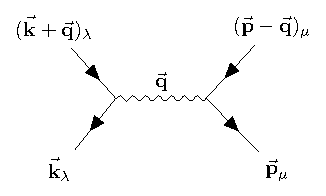
\includegraphics[width=0.55\textwidth]{../lessons/4_image/4.pdf}
\caption{\label{fig:4_3} Graphical representation of the potential energy term in second quantization.}
\end{figure}

We can easily give a graphical representation of this process.
On the bottom of Fig.\ref{fig:4_3} we can see the effect of the two destruction operators \(  a_{\va{p}\mu } a_{\va{k}\lambda } \): we destroy the two particles \( \va{k}_ \lambda  \) and \( \va{p}_ \mu  \).
Then, since we have two creation operators, as  a consequence of the Coulomb interaction \( \va{q} \), we create two particles:  \( \qty(\va{k}+\va{q})  \) with spin \( \lambda  \)  and \( \qty(\va{p}-\va{q})  \) with spin \( \mu  \). In particular, it is interesting to note that the particle with wave vector \( \va{k} \) is changed by the term \( + \va{q} \),
while the other one ,\( \va{p} \), is changed by \( \va{q} \) in such a way that the total  momentum of the system is conserved, namely by \(- \va{q} \). Hence, if one particle gains a momentum, the momentum is removed by the other in a way to be conserved, consistently with the assumption of considering a uniform system.

\end{itemize}













\end{document}
